\subsection{Complex cases}\label{app:complex-cases}

\begin{figure}[h]
  \centering
  \subfloat[High divergence]
    {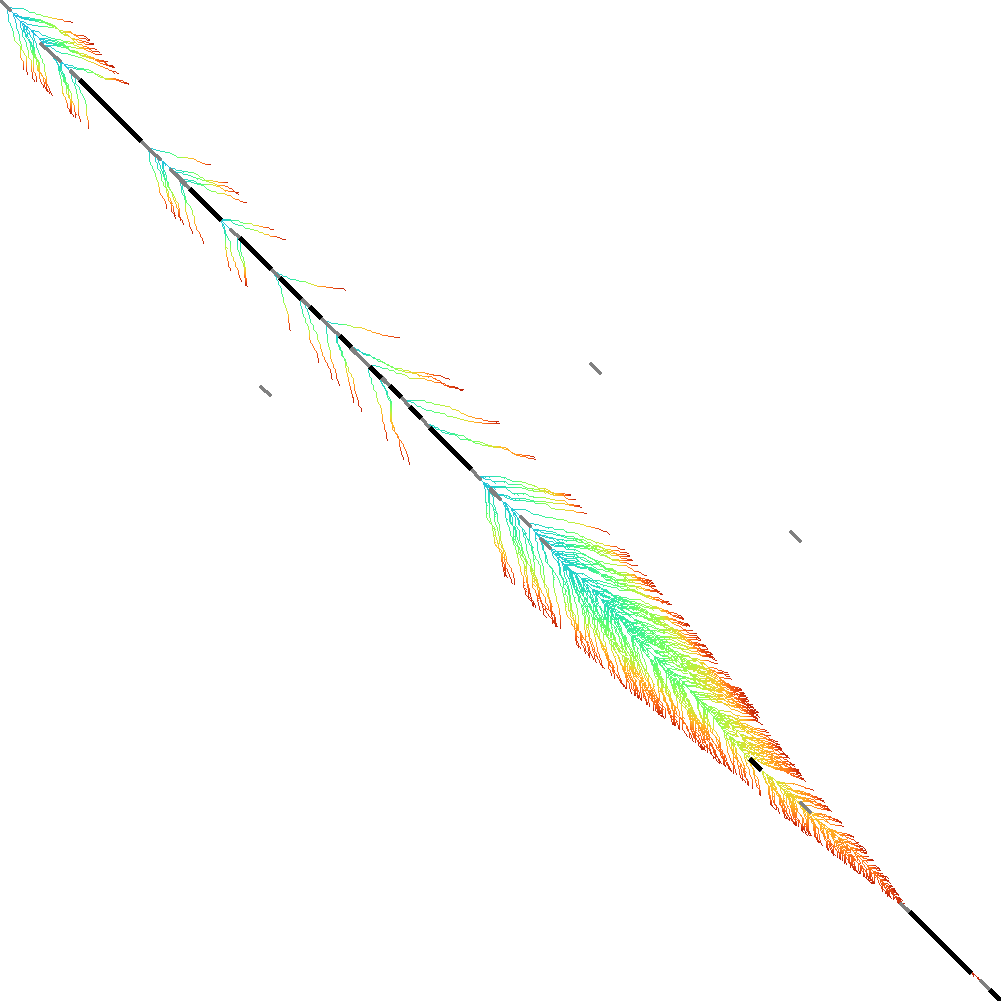
\includegraphics[height=0.31\linewidth]{imgs/limitations/high-error-rate.png}\label{fig:high_error_rate}}
  \hfill
  \subfloat[Long indel]
    {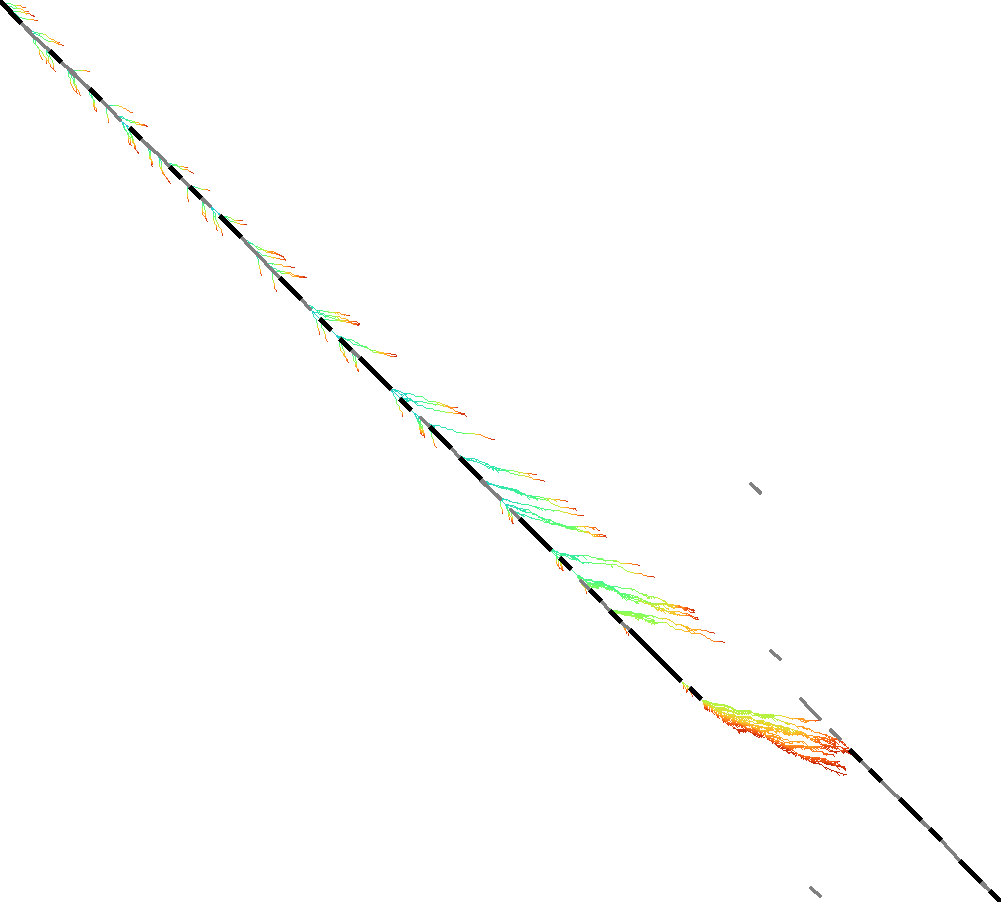
\includegraphics[height=0.31\linewidth]{imgs/limitations/deletion.png}\label{fig:deletion}}
  \hfill
  \subfloat[Short repeats]
    {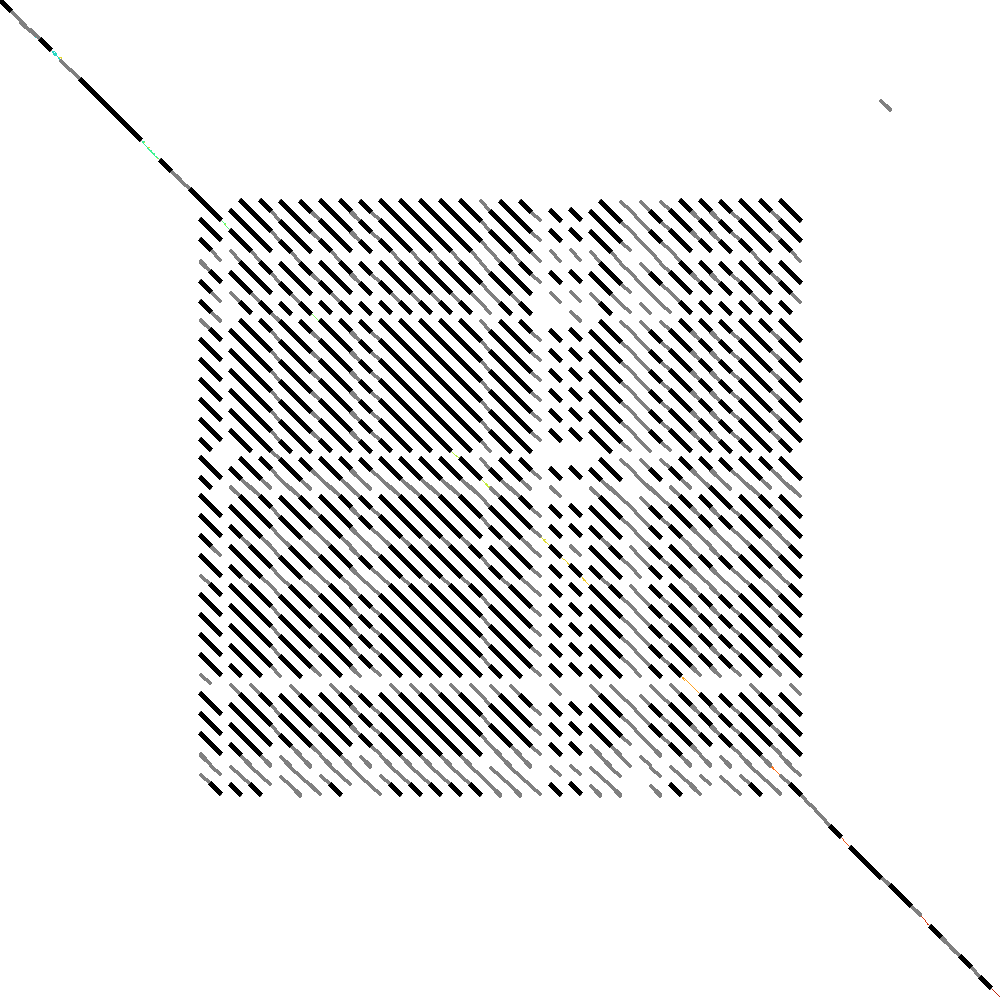
\includegraphics[height=0.31\linewidth]{imgs/limitations/repeats.png}\label{fig:repeats}}
  \caption{\textbf{Quadratic exploration behavior for complex alignments}
  (\GCH with DT, $r{=}2$, $k{=}10$, synthetic sequences, $n{=}1000$).
  \protect\subref{fig:high_error_rate} A highly divergent region, \protect\subref{fig:deletion} a deletion, and
  \protect\subref{fig:repeats} a short repeated pattern inducing a quadratic number of matches.
  The colour corresponds to the order of expansion, from \textcolor{blue}{blue}
  to \textcolor{red}{red}.}
  \label{fig:complex-cases}
\end{figure}
